\documentclass{llncs}
%
\usepackage{geometry}
\usepackage[utf8]{inputenc}
\usepackage[italian]{babel}
\usepackage{fancyhdr}
\usepackage{lipsum}
\usepackage{float}

\usepackage{hyperref}
\usepackage{graphicx}
\usepackage{wrapfig}
\usepackage{listings}
\usepackage{float}
\usepackage{bytefield}
\usepackage{algorithm}
\usepackage{algpseudocode}
\usepackage{amsmath}
\usepackage{todonotes}
\usepackage{tikz}
% LINEE GUIDA DOCUMENTAZIONE (DAL SITO DEL PROF)
%La relazione di 10 - 12 pagine, da consegnare una settimana prima dell'esame

\newcommand{\exedout}{%
	\rule{0.8\textwidth}{0.5\textwidth}%
}
\begin{document}
	\mainmatter              % start of the contributions
	%
	\title{Liar's Dice\\Sistemi Distribuiti AA 2015/2016}
	%
	\author{Davide Aguiari, Fabio Proietti}
	%
	\institute{Università di Bologna, Dipartimento di Scienze dell'Informazione
		\email{davide.aguiari@studio.unibo.it\\fabio.proietti@studio.unibo.it}}
	\maketitle
	%
%%%%%%%%%%%%%%%%%%%%%%%%%%%%%%%%%%%%%%%%%%%%%%%%%%%%%%%%%%%%%%%%%%%%%%%%%%%%%%%%%%%%%
	\begin{abstract}%-Sommario (non più di dieci righe): riassume di cosa tratta la relazione.
		Liar's Dice è un gioco da tavolo nato nel sud America e basato su un meccanismo di scommesse e bluff. Dopo una breve introduzione, andremo a spiegare quali sono state le scelte progettuali utilizzate per implementare questo passatempo, incluse l'architettura della rete, le librerie implementative e gli aspetti legati alla usabilità e correttezza del sistema.
		
	\end{abstract}

%%%%%%%%%%%%%%%%%%%%%%%%%%%%%%%%%%%%%%%%%%%%%%%%%%%%%%%%%%%%%%%%%%%%%%%%%%%%%%%%%%%%%
	\section{Introduzione}%-Introduzione: in cui si inquadra il problema affrontato, chiarendo gli obiettivi, riassumendo lo stato dell'arte, e descrivendo la struttura della relazione.
		La nostra idea di progetto è stata quella di sviluppare la versione multiplayer del  famosissimo gioco da tavolo, con un approccio di rete totalmente distribuito e attribuendo particolare attenzione all'affidabilità del sistema al fine di tollerarne i guasti di tipo crash. \\
		Liar's Dice \cite{wikiDice} è originario del Sudamerica e importato in Europa dai \textit{conquistadores} nel XV secolo. Il gioco è conosciuto anche con i nomi di \textit{Perudo}, \textit{Dudo} o, grazie anche al film Pirati dei Caraibi, come \textit{Pirate's dice}.\footnote[1]{\url{https://www.youtube.com/watch?v=piGg5ZrmoQA}}\\
		Le successive sezioni tratteranno la logica del gioco, gli aspetti progettuali, le scelte implementative adottate, la valutazione dopo la fase di test, e per finire alcune considerazioni conclusive sul sistema e possibili miglioramenti futuri.
%%%%%%%%%%%%%%%%%%%%%%%%%%%%%%%%%%%%%%%%%%%%%%%%%%%%%%%%%%%%%%%%%%%%%%%%%%%%%%%%%%%%%		 
	\section{Logica del Sistema}
		Per rendere più semplice la comprensione progettuale del sistema, in questa sezione spiegheremo più in dettaglio le regole del gioco. \\
		Ogni partita si gioca con un minimo di due giocatori ad un massimo di 8 (ma potrebbe essere superiore in base alla versione). Tutti i giocatori all'inizio di un nuovo round lanciano i dadi a loro disposizione (inizialmente sono 5) e li tengono coperti in modo che gli avversari non vedano i valori ottenuti. A questo punto colui che inizia il round, in base anche ai suoi dadi, deve effettuare una scommessa nel quale indicherà quanti dadi dello stesso numero sono potenzialmente in gioco, compresi quelli degli altri giocatori.\\ A questo punto il giocatore successivo può scegliere se credere alla precedente scommessa oppure dubitare. Nel primo caso esso è tenuto ad effettuare un rilancio sulla base dell'ultima scommessa, definendo quindi o un valore del dado maggiore rispetto al precedente oppure un numero di occorrenze superiore alla scommessa appena effettuata e passare di nuovo il turno. Nel caso in cui dubita (nella versione inglese il giocatore urla Liar!), tutti i partecipanti alla partita sveleranno i propri dadi per decretare chi ha vinto. Se la scommessa contiene un numero di occorrenze minore o uguale rispetto al valore del dado, il giocatore che ha precedentemente scommesso vince, e il suo "accusatore" perde un dado; altrimenti il vincitore sarà chi ha dubitato e a perdere un dado è lo scommettitore. Il round successivo, quindi, il giocatore perdente lancerà un dado in meno rispetto agli altri. Se un giocatore rimane senza dadi avrà automaticamente perso la partita e a vincere sarà colui che riuscirà ad eliminare tutti i partecipanti alla sfida.\\
		La nostra versione inoltre contiene anche il dado jolly: il dado di valore 1 può essere usato con un valore diverso a piacere, solo se nessuno, durante il turno, scommette utilizzando 1 come valore reale; a quel punto gli 1 smettono di valere valore jolly per tutta la durata del turno.
	
\section{Aspetti progettuali}
L'obiettivo primario del gioco progettato è la tolleranza ai guasti di tipo crash, ottenuta mediante uno studio accurato del sistema di comunicazione tra i processi giocanti e lo scambio di informazioni per mantenere la coerenza durante l'intera partita.\\

	\subsection{Il gioco}
	Il gioco (fig.\ref{board}), dal punto di vista progettuale, non differisce dalla versione realmente giocata e propone a chi gioca, una grafica accattivante e dinamica in grado di visualizzare ogni mossa fatta da ogni giocatore attivo.\\
	Ognuno è costantemente aggiornato sulla situazione dei propri dadi e di quelli degli altri, pur non vedendoli scoperti se non alla fine del turno. La board indica chi è il giocatore attivo, ovvero colui che deve far la mossa, mediante un'apposita cornice, mentre il riquadro sinistro ne riporta le informazioni in formato testuale.\\
	La logica, per ogni mossa, verifica se precedentemente vi sono già state fatte scommesse relative ai dadi sulla board: in caso negativo, significa che il giocatore attivo deve iniziare il turno e la board propone solamente la possibilità di fare una scommessa (\textit{"Make bet"}); in caso positivo il giocatore può decidere se dubitare (\textit{"Doubt"}) della scommessa del giocatore precedente, o rilanciare con una scommessa più alta, mediante gli appositi pulsanti.\\
	Il sistema, se qualcuno dubita, verifica chi ha ragione tra chi ha dubitato e il giocatore precedente che ha scommesso che sulla board c'è almeno una certa quantità di dadi con un certo valore. A questo punto chi non aveva ragione, perde uno dei 5 dadi a disposizione, mentre chi vince ha diritto a iniziare il prossimo turno.\\
	
			\begin{figure}[H]
				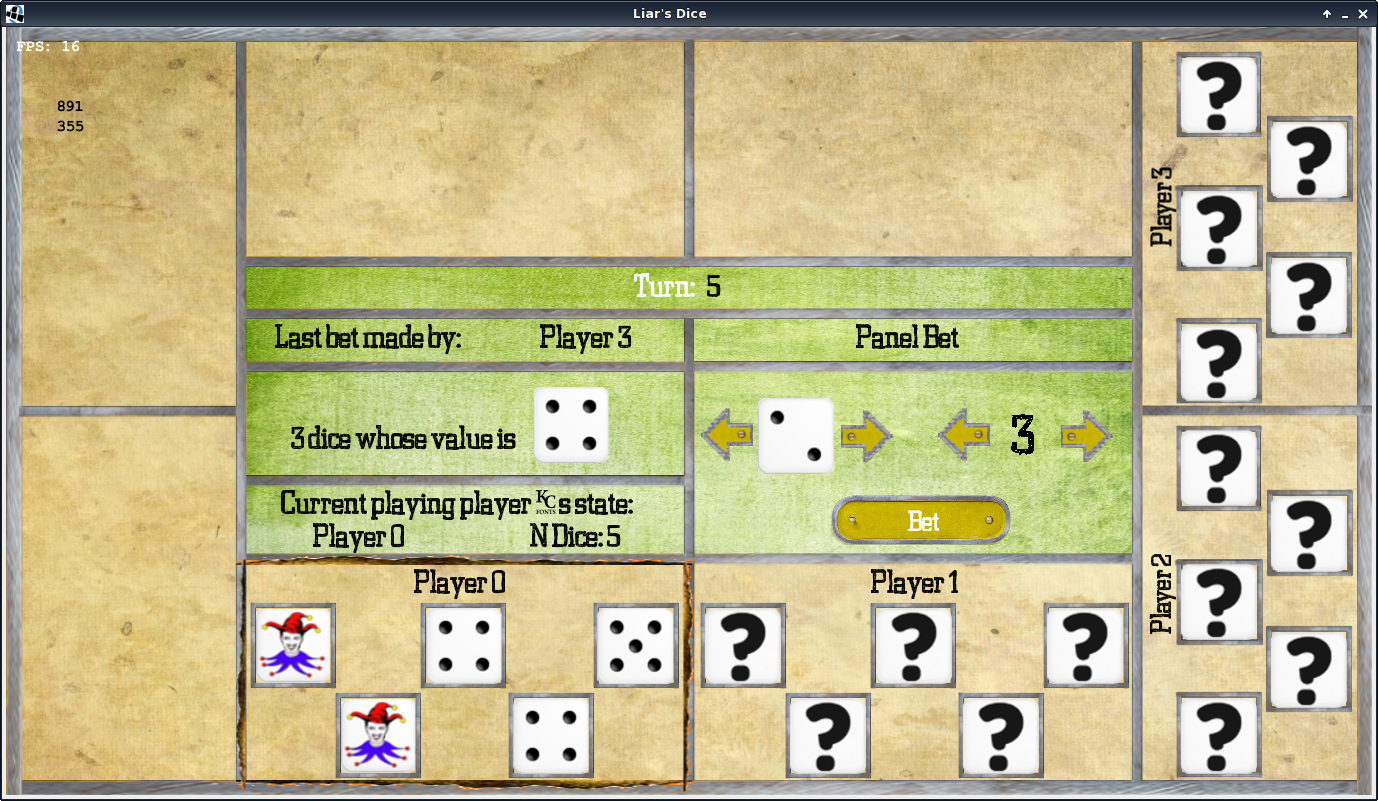
\includegraphics[scale=0.34]{img/BoardExample.png}
				\caption{\small{Screen della Board di gioco}}
				\label{board}
			\end{figure}
	
	\subsection{Connessione dei nodi con il server}
	Prima di descrivere la comunicazione tra i nodi è necessario spiegare come questi reperiscono le informazioni utili per riconoscere con chi possono interagire. \\
	Ogni nodo prima di comunicare con gli altri deve necessariamente stabilire un collegamento con una lobby che funge da server e si salva indirizzo IP e porta di ogni partecipante. Esso inizialmente attende una finestra di tempo in cui tutti i nodi possono notificare la loro volontà di connessione; al termine di questa fase, la lobby invia in broadcast un array contente gli indirizzi dei partecipanti alla partita in modo che d'ora in poi possa avvenire la comunicazione diretta solo tra nodi. Questa fase è l'unica in cui si presenta una interazione con una entità centralizzata. 

	\subsection{La comunicazione}
	L'aspetto più complesso dell'intera progettazione è stato lo studio della comunicazione tra i processi in gioco.\\
	La fasi in cui vengono scambiate le informazioni della board sono sostanzialmente tre:
	\begin{itemize}
		\item La distribuzione iniziale dei dadi
		\item La segnalazione di una mossa fatta
		\item La chiusura del turno se un giocatore dubita
	\end{itemize}
		
	\subsubsection{La distribuzione iniziale dei dadi}
	Inizialmente si era pensato di adottare un sistema di distribuzione di tipo \textit{token ring} dove ognuno creava il proprio set di dadi e, partendo da 0, possessore del token, lo si copiava nelle strutture dati apposite del successivo; successivamente anche 1, ricevuto il token da 0, poteva informare 2 dei dadi di 0 e di 1, e così via, completando quindi 2 giri del ring per avere un'informazione completa della board.\\
	Sfortunatamente si sono riscontrati alcuni problemi di latenza nello scambio dei dadi man mano che la partita proseguiva, preferendo la soluzione definitiva implementata: a inizio partita inizia sempre il giocatore con id 0 che si preoccupa di generare i dadi di tutti i giocatori connessi e di distribuirli ad ognuno, dimezzando così i messaggi richiesti per informare tutti e risolvendo i problemi riscontrati con il metodo precedente.\\
	
	\begin{figure}[H]
		\begin{minipage}{.5\textwidth}
			\centering
			\begin{tikzpicture}[->,
			main node/.style={circle,draw,thick,fill=blue!20,minimum size=4mm},
			leader node/.style={circle,draw,thick,fill=green!20,minimum size=4mm}
			]
			
			\def \n {8};
			\def \r {1.8cm};
			\def \m {11};
			
			\draw[->] (\m:\r) arc ({\m}:{360/\n -\m}:\r);
			
			\foreach \s in {1,...,\n} {
				\draw[->] ({360/\n * (\s-1) + \m}:\r) arc ({360/\n * (\s-1) + \m}:{360/\n * (\s) -\m}:\r);	
				\node[main node] at ({360/\n * (\s)}:\r) {$\s$};
			}
			\node[leader node] at (0:\r) {0};
			
			\end{tikzpicture}
		\end{minipage}
		\begin{minipage}{.5\textwidth}
			\centering
			\begin{tikzpicture}[->,
			main node/.style={circle,draw,thick,fill=blue!20,minimum size=4mm},
			leader node/.style={circle,draw,thick,fill=green!20,minimum size=4mm}
			]
			
			\def \n {8};
			\def \r {1.8cm};
			\def \m {11};
			
			%	\draw[->,gray] (\m:\r) arc ({\m}:{360/\n -\m}:\r);
			
			\foreach \s in {1,...,\n} {
				%		\draw[->,gray] ({360/\n * (\s-1) + \m}:\r) arc ({360/\n * (\s-1) + \m}:{360/\n * (\s) -\m}:\r);
				\node[main node] at ({360/\n * (\s)}:\r) (\s) {$\s$};
			}
			\node[leader node] at (0:\r) (L) {0};
			
			\draw[->] (L) to[bend right=20] (1);
			\draw[->] (L) to[bend left=5] (2);
			\draw[->] (L) to[bend left=10] (3);
			\draw[->] (L) to[bend left=1] (4);
			\draw[->] (L) to[bend right=5] (5);
			\draw[->] (L) to[bend right=10] (6);
			\draw[->] (L) to[bend right=15] (7);
			\draw[->] (L) to[bend left=20] (8);
			\end{tikzpicture}
		\end{minipage}
		\caption{\small{Primo giro, su due, dello scambio dadi con distribuzione token ring (sinistra) e  soluzione broadcast adottata (destra).}}
	\end{figure}
	
	\subsubsection{La segnalazione di una mossa fatta}
	Quando un utente ha deciso la mossa da fare (rialzare la scommessa o dubitare), il sistema notifica prima il giocatore successivo e successivamente anche tutti gli altri, così chi non è direttamente interessato alla singola puntata, conosce l'evoluzione del turno in corso.\\
	
	\begin{figure}[H]
		\begin{minipage}{.5\textwidth}
			\centering
			\begin{tikzpicture}[->,
			main node/.style={circle,draw,thick,fill=blue!20,minimum size=4mm},
			leader node/.style={circle,draw,thick,fill=green!20,minimum size=4mm}
			]
			
			\def \n {8};
			\def \r {1.8cm};
			\def \m {11};
			
			\draw[->] (\m:\r) arc ({\m}:{360/\n -\m}:\r);
			
			\foreach \s in {1,...,\n} {
				
				\node[main node] at ({360/\n * (\s)}:\r) {$\s$};
			}
			\node[leader node] at (0:\r) {0};
			
			\end{tikzpicture}
		\end{minipage}
		\begin{minipage}{.5\textwidth}
			\centering
			\begin{tikzpicture}[->,
			main node/.style={circle,draw,thick,fill=blue!20,minimum size=4mm},
			leader node/.style={circle,draw,thick,fill=green!20,minimum size=4mm}
			]
			
			\def \n {8};
			\def \r {1.8cm};
			\def \m {11};
			
			%	\draw[->,gray] (\m:\r) arc ({\m}:{360/\n -\m}:\r);
			
			\foreach \s in {1,...,\n} {
				%		\draw[->,gray] ({360/\n * (\s-1) + \m}:\r) arc ({360/\n * (\s-1) + \m}:{360/\n * (\s) -\m}:\r);
				\node[main node] at ({360/\n * (\s)}:\r) (\s) {$\s$};
			}
			\node[leader node] at (0:\r) (L) {0};
			
			\draw[->] (L) to[bend left=5] (2);
			\draw[->] (L) to[bend left=10] (3);
			\draw[->] (L) to[bend left=1] (4);
			\draw[->] (L) to[bend right=5] (5);
			\draw[->] (L) to[bend right=10] (6);
			\draw[->] (L) to[bend right=15] (7);
			\draw[->] (L) to[bend left=20] (8);
			\end{tikzpicture}
		\end{minipage}
		\caption{\small{Il giocatore 0 fa una scommessa e la segnala a 1 indicandogli che sarà il prossimo a dover giocare (sinistra); il giocatore 0 notifica a tutti la propria scommessa (destra).}}
	\end{figure}

		\subsubsection{La chiusura del turno se un giocatore dubita}
		Nel momento in cui un giocatore dubita, il turno finisce. Il sistema verifica se il giocatore in questione ha ragione o torto ad aver dubitato. In ogni caso sarà questo giocatore ad avvisare tutti dell'esito del dubbio, rigenerando tutti i dadi e notificando in broadcast come si è concluso il turno.
		
		\begin{figure}[H]
			
			\centering
			\begin{tikzpicture}[->,
			main node/.style={circle,draw,thick,fill=blue!20,minimum size=4mm},
			leader node/.style={circle,draw,thick,fill=red!50,minimum size=4mm},
			winning node/.style={circle,draw,thick,fill=green!50,minimum size=4mm}
			]
			
			\def \n {8};
			\def \r {1.8cm};
			\def \m {11};
			
			%	\draw[->,gray] (\m:\r) arc ({\m}:{360/\n -\m}:\r);
			
			\foreach \s in {2,...,\n} {
				%		\draw[->,gray] ({360/\n * (\s-1) + \m}:\r) arc ({360/\n * (\s-1) + \m}:{360/\n * (\s) -\m}:\r);
				\node[main node] at ( {360/\n * (\s)}:\r) (\s) {$\s$};
			}
			\node[winning node] at ({360/\n * (1)}:\r) (W) {1};
			\node[leader node] at (0:\r) (L) {0};
			
			\draw[->] (W) to[bend left=5] (2);
			\draw[->] (W) to[bend left=10] (3);
			\draw[->] (W) to[bend left=1] (4);
			\draw[->] (W) to[bend right=5] (5);
			\draw[->] (W) to[bend right=10] (6);
			\draw[->] (W) to[bend right=15] (7);
			\draw[->] (W) to[bend left=20] (8);
			\end{tikzpicture}
			\caption{\small{Il giocatore 1 dubita della scommessa del giocatore 0, vince il turno; rigenera i dadi e li distribuisce a tutti notificando l'esito del turno precedente}}
		\end{figure}

\subsection{La tolleranza ai guasti}

La tolleranza ai guasti di tipo crash è stata progettata come segue:\\
se un giocatore in attesa del proprio turno va in crash, il primo processo che interagisce con lui\footnote{Interagisce per notificargli una mossa effettuata o la fine di un turno o l'utilizzo del jolly ecc.} si accorge e notifica a tutti l'evento crash; a questo punto il gioco continua tenendo conto del set di dadi del player in crash fino alla fine del turno.\\
Se, invece, il giocatore con il controllo del turno va in crash, tutti vengono automaticamente notificati dell'evento e sarà il giocatore con id successivo a continuare il gioco.


\begin{figure}[H]
	\begin{minipage}{0.45\textwidth}
		\centering
		\begin{tikzpicture}[->,
		main node/.style={circle,draw,thick,fill=blue!20,minimum size=4mm},
		crashed node/.style={circle,draw,thick,fill=red!50,minimum size=4mm}
		]
		
		\def \n {8};
		\def \r {1.8cm};
		\def \m {11};
		
		\draw[->,gray] (\m:\r) arc ({\m}:{360/\n -\m}:\r);
		
		\foreach \s in {1,...,\n} {
			\draw[->,gray] ({360/\n * (\s-1) + \m}:\r) arc ({360/\n * (\s-1) + \m}:{360/\n * (\s) -\m}:\r);
			\node[main node] at ({360/\n * (\s)}:\r) (\s) {$\s$};
		}
		\node[crashed node] at (0:\r) (L) {0};
		
		\draw[->] (1) to[bend right=20] (L);
		\draw[->] (2) to[bend right=20] (L);
		\draw[->] (3) to[bend right=10] (L);
		\draw[->] (4) to[bend left=10] (L);
		\draw[->] (5) to[bend left=20] (L);
		\draw[->] (6) to[bend left=20] (L);
		\draw[->] (7) to[bend left=20] (L);
		\draw[->] (8) to[bend left=20] (L);
		\end{tikzpicture}
	\end{minipage}
	\begin{minipage}{0.45\textwidth}
		\centering
		\begin{tikzpicture}[->,
		main node/.style={circle,draw,thick,fill=blue!20,minimum size=4mm},
		crashed node/.style={circle,draw,thick,fill=gray,minimum size=4mm},
		leader node/.style={circle,draw,thick,fill=green!20,minimum size=4mm}
		]
		
		\def \n {8};
		\def \r {1.8cm};
		\def \m {11};
		
		
		\draw[->,gray] ({360/\n * (2-1) + \m}:\r) arc ({360/\n * (2-1) + \m}:{360/\n * (2) -\m}:\r);
		\node[leader node] at ({360/\n * (2-1)}:\r) (2) {$1$};
		
		\draw[->,gray] ({360/\n * (3-1) + \m}:\r) arc ({360/\n * (3-1) + \m}:{360/\n * (3) -\m}:\r);
		\node[main node] at ({360/\n * (3-1)}:\r) (3) {$2$};
		
		\draw[->,gray] ({360/\n * (4-1) + \m}:\r) arc ({360/\n * (4-1) + \m}:{360/\n * (4) -\m}:\r);
		\node[main node] at ({360/\n * (4-1)}:\r) (4) {$3$};
		
		\draw[->,gray] ({360/\n * (5-1) + \m}:\r) arc ({360/\n * (5-1) + \m}:{360/\n * (5) -\m}:\r);
		
		\node[main node] at ({360/\n * (5-1)}:\r) (5) {$4$};
		
		\draw[->,gray] ({360/\n * (6-1) + \m}:\r) arc ({360/\n * (6-1) + \m}:{360/\n * (6) -\m}:\r);
		\node[main node] at ({360/\n * (6-1)}:\r) (6) {$5$};
		
		\draw[->,gray] ({360/\n * (7-1) + \m}:\r) arc ({360/\n * (7-1) + \m}:{360/\n * (7) -\m}:\r);
		\node[main node] at ({360/\n * (7-1)}:\r) (7) {$6$};
		%			
		%			\draw[->,gray] ({360/\n * (8-1) + \m}:\r) arc ({360/\n * (8-1) + \m}:{360/\n * (8) -\m}:\r);
		\node[main node] at ({360/\n * (8-1)}:\r) (8) {$7$};
		
		\draw[->,gray] (8) to [bend right=80] (1);
		
		\node[crashed node] at (0:\r) (L) {0};
		\draw[->] (3) to[bend right=10] (1);
		\draw[->] (4) to[bend left=10] (1);
		\draw[->] (5) to[bend left=20] (1);
		\draw[->] (6) to[bend left=20] (1);
		\draw[->] (7) to[bend left=20] (1);
		\draw[->] (8) to[bend left=20] (1);
		\end{tikzpicture}
	\end{minipage}
	\caption{\small{Riconfigurazione dei giocatori dopo un crash del giocatore con il controllo del turno}}
\end{figure}
E' chiaro quindi come il crash di un client non inficia lo sviluppo di un turno, dato che tutti conoscono i dadi degli altri e il sistema permette di concludere la scommessa senza bisogno di un restart del turno. Quest'ultimo avviene solo nel caso in cui sia il crash avvenga per il giocatore che sta generando i dadi di tutti: questo particolare caso può essere presente in due distinte fasi dell'intera partita:
\begin{itemize}
	\item A inizio partita, dopo che ogni giocatore conosce gli altri, può capitare che il giocatore con id 0 sia in crash, non permettendo agli altri di iniziare il turno. E' stato impostato un timeout di tempo arbitrario, per notificare a tutti l'anomalia; a questo punto il giocatore con id successivo si farà carico di ridistribuire i dadi e di verificare la reale situazione del giocatore 0.
	\item A inizio turno successivo al primo della partita, il giocatore che ha vinto può essere in crash prima o dopo aver notificato l'esito; se il crash avviene prima, l'esito viene annullato e il giocatore successivo continua come nessuno avesse dubitato, mentre se avviene dopo allora il giocatore successivo prende il controllo del turno rigenerando i dadi per tutti.
\end{itemize}
		\begin{figure}[H]
			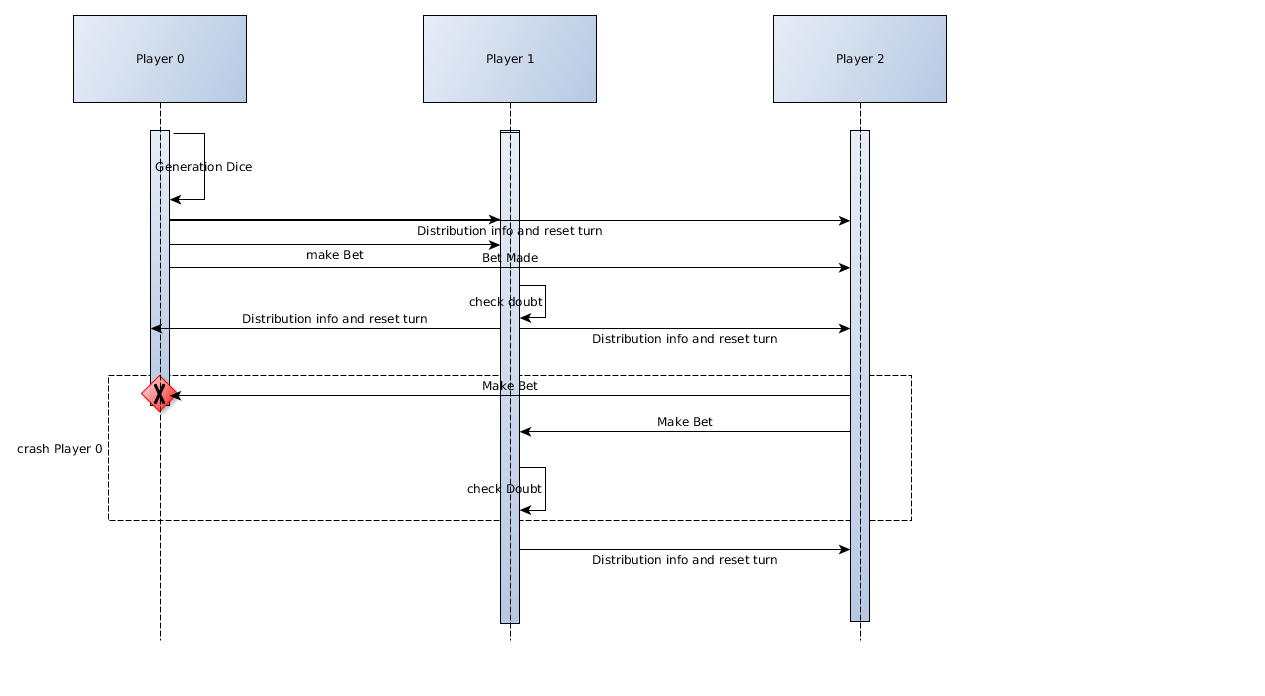
\includegraphics[scale=0.34]{img/Activity.png}
			\caption{\small{Activity Diagram di 3 giocatori e con presenza di crash.}}
			\label{activity}
		\end{figure}
	\newpage
%%%%%%%%%%%%%%%%%%%%%%%%%%%%%%%%%%%%%%%%%%%%%%%%%%%%%%%%%%%%%%%%%%%%%%%%%%%%%%%%%%%%%	
	\section{Aspetti Implementativi}%-Aspetti implementativi: dettagli sulle scelte implementative, ed architettura specifica implementata. Inserire almeno il diagramma delle classi e uno delle interazioni secondo lo standard UML.
		\subsection{Design Pattern}
			La nostra implementazione si è subito orientata sull'utilizzo del design pattern Model View Controller\cite{MVC}. MVC si sposa perfettamente con le nostre esigenze: la parte che costituisce il Model infatti gestisce direttamente i dati, la logica e le regole del gioco; la View ha lo scopo di mostrare le informazioni elaborate (e quindi l'output grafico) all'utente, che tramite il Controller è in grado di manipolare.
			
		\subsection{Implementazione della logica del gioco}
			La figura \ref{Model} mostra il digramma UML delle classi utilizzate per implementare la logica della nostra applicazione. Lo scopo del Model è quindi quello di generare i giocatori, i dadi, verificare le scommesse e riorganizzare lo stato dello stesso in caso di guasti improvvisi. La classe DiceLiar, oltre a far connettere tra di loro i processi, ha lo scopo di definire l'oggetto \textit{board}. Essa attraverso gli oggetti delle classi \textit{Dice}, \textit{Players} e \textit{Bet} gestisce il game loop e l'aggiornamento degli elementi.
			\newpage
			\begin{figure}[H]
				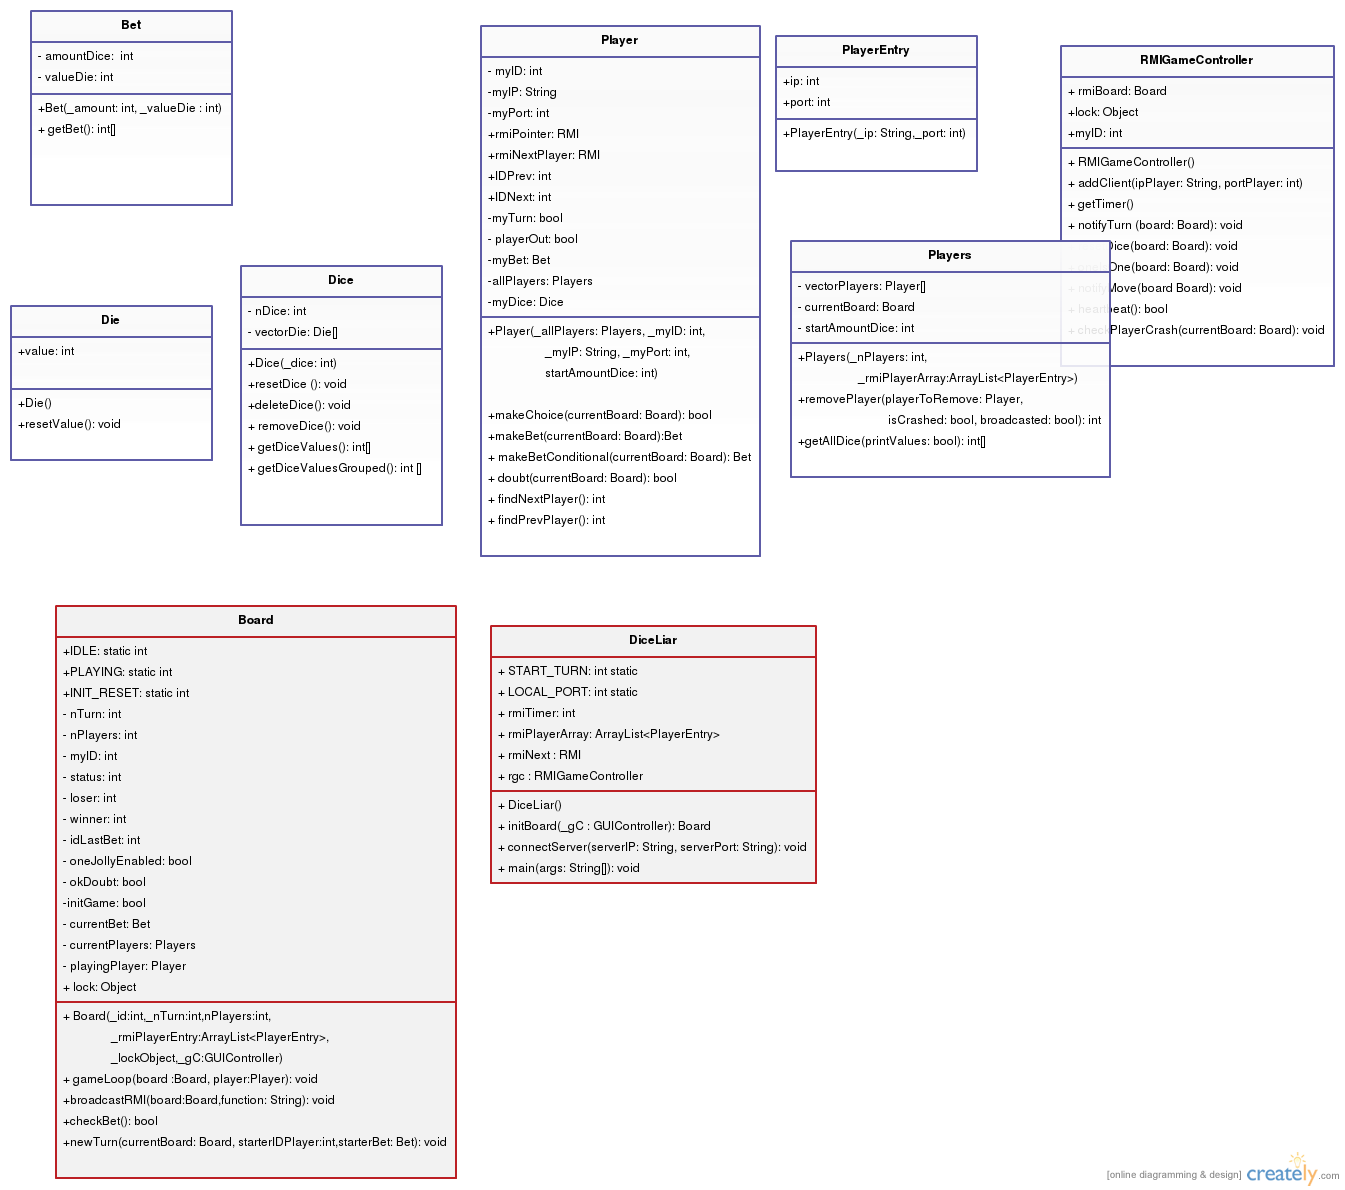
\includegraphics[scale=0.35]{img/Model.png}
				\caption{\small{Class Diagram della componente Model.}}
				\label{Model}
			\end{figure}
			\newpage
		\subsection{L'interfaccia grafica}
			Per l'implementazione dell'interfaccia grafica ci siamo affidati alla libreria Open Source Slick2D \cite{Slick}. E' formata da un insieme di tools e funzionalità basate sulle librerie grafiche OpenGL e LWJGL, offrendo quindi un supporto per includere animazioni, immagini, suoni, ecc. alla nostra grafica 2D. L'utilizzo di Slick2D passa attraverso l'implementazione di una classe principale che ha lo scopo di gestire tutte le caratteristiche principali della view come il frame rate, la grandezza della finestra, la modalità di rendering, il passaggio di stato ecc. Tutte le classi che invece definiscono gli stati del sistema, si basano su tre metodi principali: 
				\begin{itemize}
					\item void init(): è il metodo richiamato al lancio dell'interfaccia e serve principalmente per l'inizializzazione e il caricamento degli elementi;
					\item void update(): è un metodo ciclico che aggiorna costantemente lo stato degli elementi inizializzati dal precedente metodo attraverso le informazioni generate dalla componente Controller;
					\item void render(): in base al refresh rate definito nella classe principale mostra gli elementi disegnati costantemente aggiornati.
				\end{itemize}
			L'intero processo della view è eseguito su un thread dedicato. La classe Main si occupa di gestire i vari stati in base alle interazioni che l'utente ha con essa.
			Per quanto riguarda gli aggiornamenti grafici (dadi correnti, ultima scommessa, ecc.) la view (fig.\ref*{View}) utilizza i valori definiti nella classe \textit{GUIController}, che appunto funge da controller (fig.\ref{Controller}).
		\begin{figure}[H]
			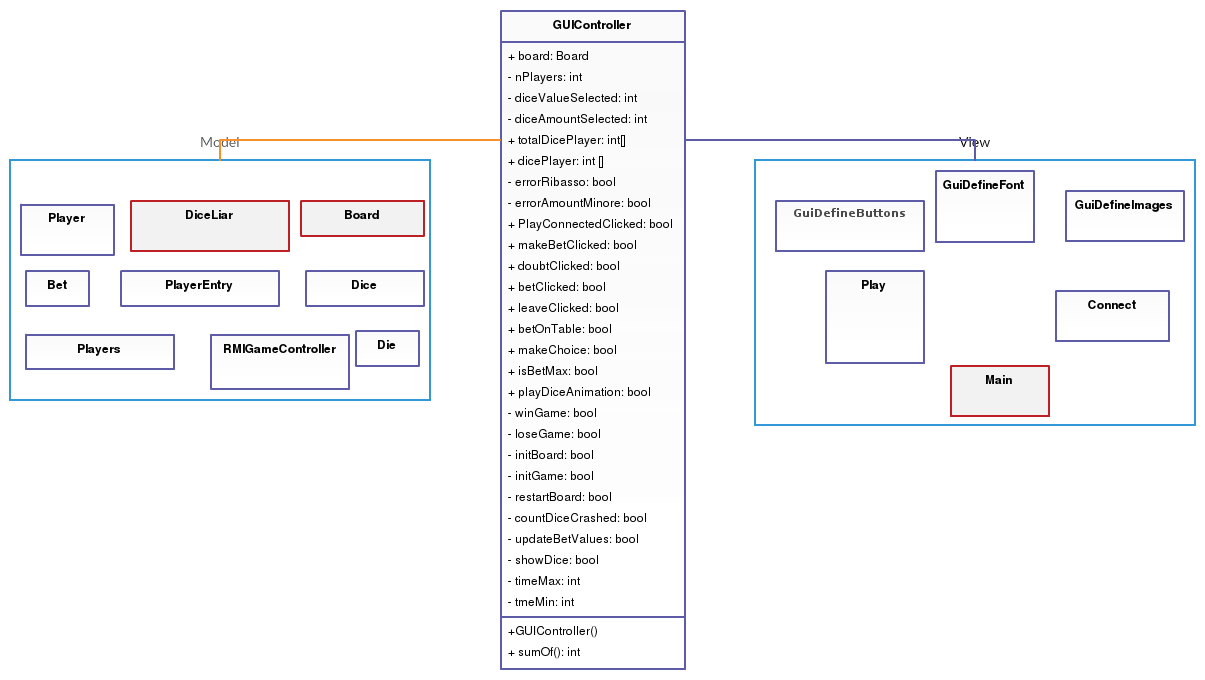
\includegraphics[scale=0.34]{img/Controller.png}
			\caption{\small{Class Diagram della componente Controller.}}
			\label{Controller}
		\end{figure}	
		\newpage
		\begin{figure}[H]
			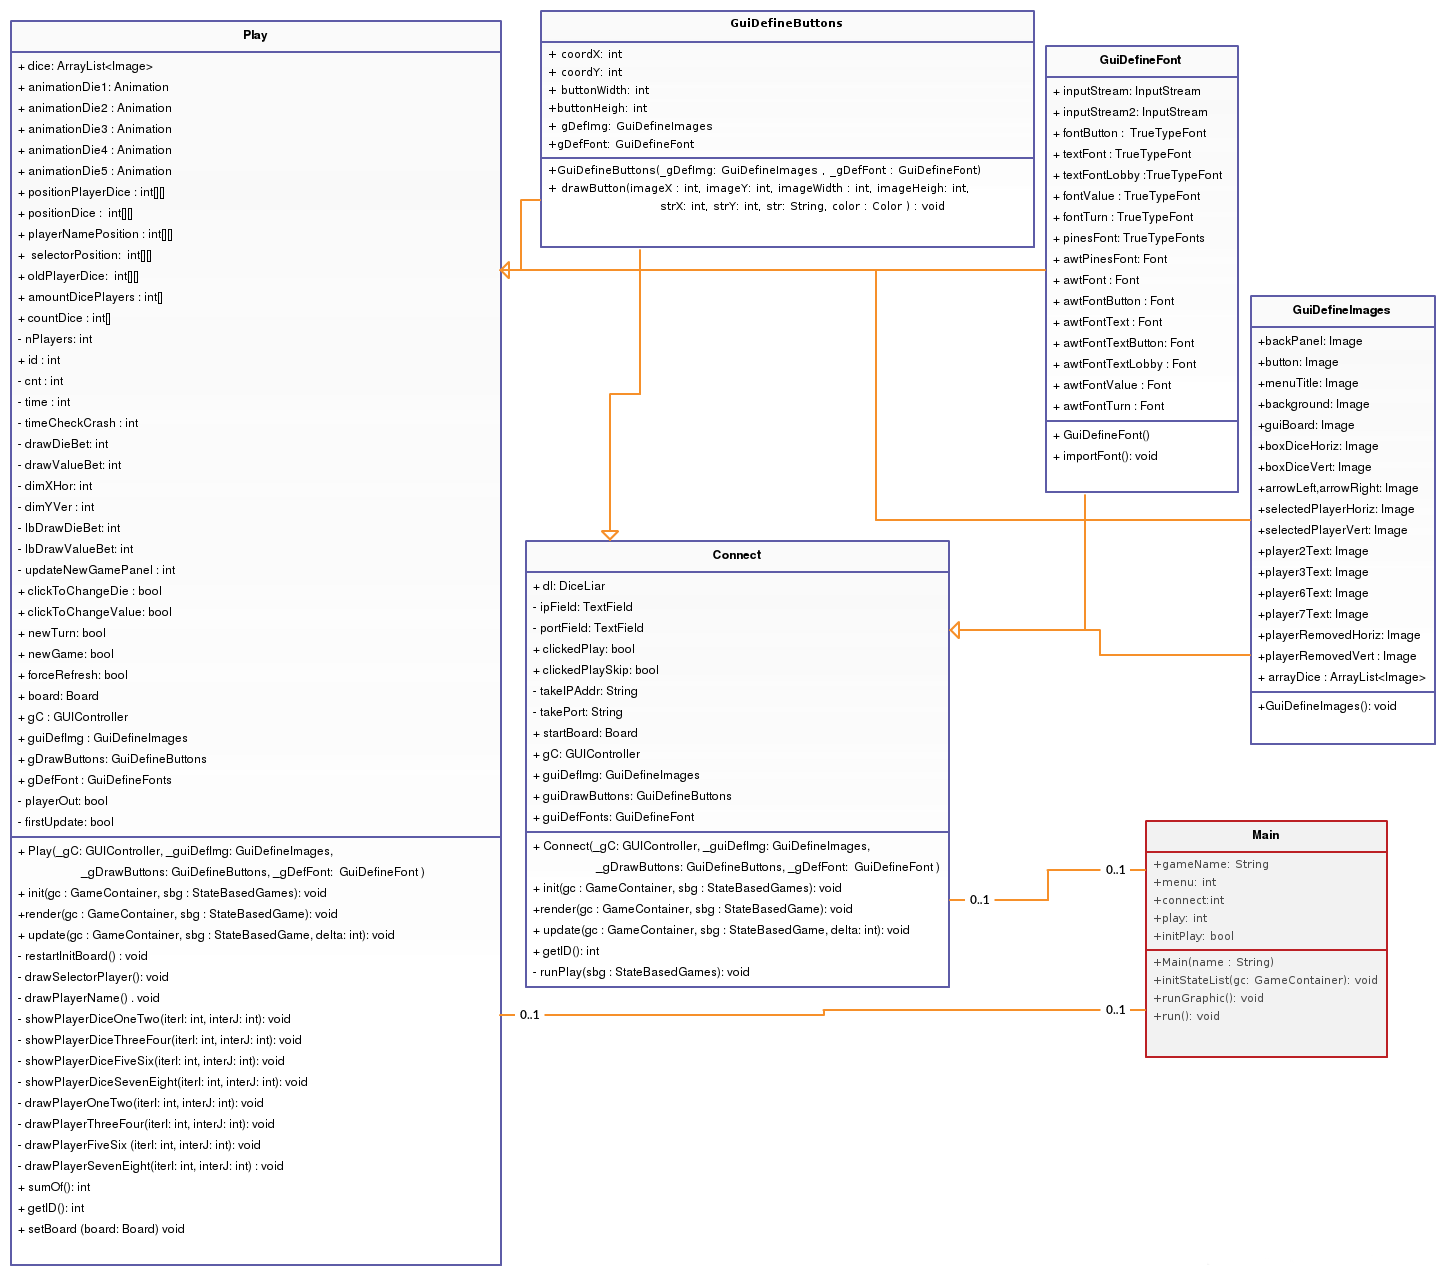
\includegraphics[scale=0.34]{img/View.png}
			\caption{\small{Class Diagram della componente View.}}
			\label{View}
		\end{figure}
		
		\subsection{Comunicazione tra nodi}
			Lo scambio di informazioni tra i nodi distribuiti viene effettuato attraverso le API di java RMI. La Remote Method Invocation infatti permette a tutti i processi di invocare dei metodi remoti, fornendo così omogeneità e simmetria nel progetto; infatti la procedura utilizzata è disegnata sul paradadigma Object Oriented e i vari processi si comportano come degli oggetti che effettuano delle chiamate a metodi.
			Più precisamente ogni nodo presente in una differente Virtual Machine, ha 
			l'obbligo di implementare una interfaccia comune a tutti gli altri che mostra quali metodi sono "esportabili". 
			In generale RMI è composto da 3 entità distinte: 
				\begin{itemize}
					\item Uno o più server RMI;
					\item Uno o più client RMI;
					\item Uno o più Java RMI Registry (uno per ogni server).
				\end{itemize}
			Il processo che funge da server implementa l'interfaccia relativa agli oggetti che intende esportare e li registra nel proprio registry, che non è altro che un processo demone che tiene traccia di questi oggetti. Il client quindi non fa altro che effettuare delle chiamate a questo registro al fine di utilizzarne gli oggetti presenti. La gestione della comunicazione è affidata allo stub \cite{rmi}. \\
			Nel caso di Liar's Dice abbiamo deciso di implementare questa tecnica in modo che ogni nodo funga sia da client che da server traedone molteplici vantaggi, uno su tutti la possibilità definire la politica di tolleranza ai guasti descritta precedentemente.
			
%%%%%%%%%%%%%%%%%%%%%%%%%%%%%%%%%%%%%%%%%%%%%%%%%%%%%%%%%%%%%%%%%%%%%%%%%%%%%%%%%%%%%	


	
%%%%%%%%%%%%%%%%%%%%%%%%%%%%%%%%%%%%%%%%%%%%%%%%%%%%%%%%%%%%%%%%%%%%%%%%%%%%%%%%%%%%%	
	\section{Valutazione e Conclusioni}%-Valutazione: confronto delle soluzioni proposte con soluzioni analoghe allo stato dell'arte.
	%-Conclusioni: commenti conclusivi su possibili miglioramenti di quanto discusso, e possibili linee di intervento futuro.
		La fase più importante per trarre le nostre conclusioni è stata quella di testing; infatti nel momento in cui abbiamo avuto la nesessità di apportate delle modifiche al codice, siamo stati costretti a rivedere alcune scelte implementative stabilite precedentemente. Dato che la nostra prima implementazione del design pattern MVC non era di facile gestione, abbiamo deciso di raffinare la sua struttura introducendo specifiche classi "ponte" contenenti tutti gli elementi necessari all'aggiornamento sia del model che della view. \\
		Il progetto ha richiesto circa 1 mese/uomo e si è dimostrato ostico nella configurazione iniziale di RMI e nella risoluzione del bug nella distribuzione dei dadi iniziale che portava la CPU al ~700\% facendoci preferire una modalità diversa, di tipo broadcast.
		Il lavoro di bugfix è stato importante anche per l'introduzione di alcune migliorie grafiche che hanno migliorato l'esperienza di gioco dell'utente. \\
		In conclusione, visto lo stato attuale del progetto, vi è la possibilità di estenderlo con features quali la modalità di gioco single player o un più semplice meccanismo di connessione al server. Infine la grande versatilità di java potrebbe favorire una semplice e fluida esperienza di gioco sia in ambienti mobile che desktop.
	

%%%%%%%%%%%%%%%%%%%%%%%%%%%%%%%%%%%%%%%%%%%%%%%%%%%%%%%%%%%%%%%%%%%%%%%%%%%%%%%%%%%%%
	\begin{thebibliography}{}
		\bibitem{wikiDice} \url{https://en.wikipedia.org/wiki/Liar's\_dice}
		\bibitem{MVC} \url{https://en.wikipedia.org/wiki/Model%E2%80%93view%E2%80%93controller}
		\bibitem{Slick} \url{http://slick.ninjacave.com/}
		\bibitem{rmi} \url{https://docs.oracle.com/javase/tutorial/rmi/}
	\end{thebibliography}
\end{document}